% Options for packages loaded elsewhere
\PassOptionsToPackage{unicode}{hyperref}
\PassOptionsToPackage{hyphens}{url}
\PassOptionsToPackage{dvipsnames,svgnames,x11names}{xcolor}
%
\documentclass[
  letterpaper,
  DIV=11,
  numbers=noendperiod]{scrartcl}

\usepackage{amsmath,amssymb}
\usepackage{lmodern}
\usepackage{iftex}
\ifPDFTeX
  \usepackage[T1]{fontenc}
  \usepackage[utf8]{inputenc}
  \usepackage{textcomp} % provide euro and other symbols
\else % if luatex or xetex
  \usepackage{unicode-math}
  \defaultfontfeatures{Scale=MatchLowercase}
  \defaultfontfeatures[\rmfamily]{Ligatures=TeX,Scale=1}
\fi
% Use upquote if available, for straight quotes in verbatim environments
\IfFileExists{upquote.sty}{\usepackage{upquote}}{}
\IfFileExists{microtype.sty}{% use microtype if available
  \usepackage[]{microtype}
  \UseMicrotypeSet[protrusion]{basicmath} % disable protrusion for tt fonts
}{}
\makeatletter
\@ifundefined{KOMAClassName}{% if non-KOMA class
  \IfFileExists{parskip.sty}{%
    \usepackage{parskip}
  }{% else
    \setlength{\parindent}{0pt}
    \setlength{\parskip}{6pt plus 2pt minus 1pt}}
}{% if KOMA class
  \KOMAoptions{parskip=half}}
\makeatother
\usepackage{xcolor}
\usepackage[margin=1in]{geometry}
\setlength{\emergencystretch}{3em} % prevent overfull lines
\setcounter{secnumdepth}{-\maxdimen} % remove section numbering
% Make \paragraph and \subparagraph free-standing
\ifx\paragraph\undefined\else
  \let\oldparagraph\paragraph
  \renewcommand{\paragraph}[1]{\oldparagraph{#1}\mbox{}}
\fi
\ifx\subparagraph\undefined\else
  \let\oldsubparagraph\subparagraph
  \renewcommand{\subparagraph}[1]{\oldsubparagraph{#1}\mbox{}}
\fi


\providecommand{\tightlist}{%
  \setlength{\itemsep}{0pt}\setlength{\parskip}{0pt}}\usepackage{longtable,booktabs,array}
\usepackage{calc} % for calculating minipage widths
% Correct order of tables after \paragraph or \subparagraph
\usepackage{etoolbox}
\makeatletter
\patchcmd\longtable{\par}{\if@noskipsec\mbox{}\fi\par}{}{}
\makeatother
% Allow footnotes in longtable head/foot
\IfFileExists{footnotehyper.sty}{\usepackage{footnotehyper}}{\usepackage{footnote}}
\makesavenoteenv{longtable}
\usepackage{graphicx}
\makeatletter
\def\maxwidth{\ifdim\Gin@nat@width>\linewidth\linewidth\else\Gin@nat@width\fi}
\def\maxheight{\ifdim\Gin@nat@height>\textheight\textheight\else\Gin@nat@height\fi}
\makeatother
% Scale images if necessary, so that they will not overflow the page
% margins by default, and it is still possible to overwrite the defaults
% using explicit options in \includegraphics[width, height, ...]{}
\setkeys{Gin}{width=\maxwidth,height=\maxheight,keepaspectratio}
% Set default figure placement to htbp
\makeatletter
\def\fps@figure{htbp}
\makeatother
\newlength{\cslhangindent}
\setlength{\cslhangindent}{1.5em}
\newlength{\csllabelwidth}
\setlength{\csllabelwidth}{3em}
\newlength{\cslentryspacingunit} % times entry-spacing
\setlength{\cslentryspacingunit}{\parskip}
\newenvironment{CSLReferences}[2] % #1 hanging-ident, #2 entry spacing
 {% don't indent paragraphs
  \setlength{\parindent}{0pt}
  % turn on hanging indent if param 1 is 1
  \ifodd #1
  \let\oldpar\par
  \def\par{\hangindent=\cslhangindent\oldpar}
  \fi
  % set entry spacing
  \setlength{\parskip}{#2\cslentryspacingunit}
 }%
 {}
\usepackage{calc}
\newcommand{\CSLBlock}[1]{#1\hfill\break}
\newcommand{\CSLLeftMargin}[1]{\parbox[t]{\csllabelwidth}{#1}}
\newcommand{\CSLRightInline}[1]{\parbox[t]{\linewidth - \csllabelwidth}{#1}\break}
\newcommand{\CSLIndent}[1]{\hspace{\cslhangindent}#1}

\usepackage{booktabs}
\usepackage{longtable}
\usepackage{array}
\usepackage{multirow}
\usepackage{wrapfig}
\usepackage{float}
\usepackage{colortbl}
\usepackage{pdflscape}
\usepackage{tabu}
\usepackage{threeparttable}
\usepackage{threeparttablex}
\usepackage[normalem]{ulem}
\usepackage{makecell}
\usepackage{xcolor}
\usepackage{xr}
\usepackage[default]{sourcesanspro}
\usepackage{sourcecodepro}
\usepackage{lineno}
\linenumbers
\KOMAoption{captions}{tableheading}
\makeatletter
\makeatother
\makeatletter
\makeatother
\makeatletter
\@ifpackageloaded{caption}{}{\usepackage{caption}}
\AtBeginDocument{%
\ifdefined\contentsname
  \renewcommand*\contentsname{Table of contents}
\else
  \newcommand\contentsname{Table of contents}
\fi
\ifdefined\listfigurename
  \renewcommand*\listfigurename{List of Figures}
\else
  \newcommand\listfigurename{List of Figures}
\fi
\ifdefined\listtablename
  \renewcommand*\listtablename{List of Tables}
\else
  \newcommand\listtablename{List of Tables}
\fi
\ifdefined\figurename
  \renewcommand*\figurename{Figure}
\else
  \newcommand\figurename{Figure}
\fi
\ifdefined\tablename
  \renewcommand*\tablename{Table}
\else
  \newcommand\tablename{Table}
\fi
}
\@ifpackageloaded{float}{}{\usepackage{float}}
\floatstyle{ruled}
\@ifundefined{c@chapter}{\newfloat{codelisting}{h}{lop}}{\newfloat{codelisting}{h}{lop}[chapter]}
\floatname{codelisting}{Listing}
\newcommand*\listoflistings{\listof{codelisting}{List of Listings}}
\makeatother
\makeatletter
\@ifpackageloaded{caption}{}{\usepackage{caption}}
\@ifpackageloaded{subcaption}{}{\usepackage{subcaption}}
\makeatother
\makeatletter
\@ifpackageloaded{tcolorbox}{}{\usepackage[many]{tcolorbox}}
\makeatother
\makeatletter
\@ifundefined{shadecolor}{\definecolor{shadecolor}{rgb}{.97, .97, .97}}
\makeatother
\makeatletter
\makeatother
\ifLuaTeX
  \usepackage{selnolig}  % disable illegal ligatures
\fi
\IfFileExists{bookmark.sty}{\usepackage{bookmark}}{\usepackage{hyperref}}
\IfFileExists{xurl.sty}{\usepackage{xurl}}{} % add URL line breaks if available
\urlstyle{same} % disable monospaced font for URLs
\hypersetup{
  colorlinks=true,
  linkcolor={blue},
  filecolor={Maroon},
  citecolor={Blue},
  urlcolor={Blue},
  pdfcreator={LaTeX via pandoc}}

\author{}
\date{}

\begin{document}
\ifdefined\Shaded\renewenvironment{Shaded}{\begin{tcolorbox}[borderline west={3pt}{0pt}{shadecolor}, enhanced, breakable, boxrule=0pt, interior hidden, sharp corners, frame hidden]}{\end{tcolorbox}}\fi

\newpage

How LMA of understory plants responses to artificial light at night

\[ \]

Cong Zhou\textsuperscript{1,2}, Akihiro Nakamura\textsuperscript{1},
Masatoshi Katabuchi\textsuperscript{1},

\[ \]

\textsuperscript{1} CAS Key Laboratory of Tropical Forest Ecology,
Xishuangbanna Tropical Botanical Garden, Chinese Academy of Sciences,
Menglun, Yunnan 666303, China

\textsuperscript{2} University of Chinese Academy of Sciences, Beijing
100049, China

\[ \]

\textbf{Corresponding Author}:

Masatoshi Katabuchi

E-mail: katabuchi@xtbg.ac.cn; mattocci27@gmail.com

\[ \]

\textbf{Running title}:

\newpage

\hypertarget{abstract}{%
\section{ABSTRACT}\label{abstract}}

\textbf{KEY WORDS} light pollution, leaf mass per area (LMA), leaf
punch, Artificial light at night (ALAN)

\hypertarget{introduction}{%
\section{INTRODUCTION}\label{introduction}}

Light pollution caused by artificial light at night (ALAN) has disturbed
ecological processes since the start of 20th century
(\protect\hyperlink{ref-Longcore2004}{Longcore and Rich 2004};
\protect\hyperlink{ref-Gaston2013}{Gaston et al. 2013};
\protect\hyperlink{ref-Bennie2016}{Bennie et al. 2016}). Artificial
light at night extends both in intensity covered a large illuminance
range from the degree hard to detect to almost daylight and in extent
covered more and more World's terrestrial surfaces
(\protect\hyperlink{ref-Bennie2016}{Bennie et al. 2016};
\protect\hyperlink{ref-Falchi2016}{2016}). ALAN influences behavior or
physiology of a wide broad range of taxonomic groups including mammals,
birds, reptiles, amphibians, fishes, invertebrates, and plants
(\protect\hyperlink{ref-Rich2006}{Rich and Longcore 2006}). For example,
ALAN attracts insects interfering in movement, foraging, reproduction,
development so as an important bringer to drive insects population
decline (\protect\hyperlink{ref-Owens2020}{Owens et al. 2020};
\protect\hyperlink{ref-Boyes2021}{Boyes et al. 2021}). Although many
studies have focused on how ALAN change the behavior of animals
(\protect\hyperlink{ref-Russart2018}{Russart and Nelson 2018}), its
influence on plants has also received attentions {[}Speißer, Liu, and
van Kleunen (\protect\hyperlink{ref-Speisser2021a}{2021});
(\protect\hyperlink{ref-Liu2022}{\textbf{Liu2022?}}); Matthew effect{]}.
A recent studies experimentally showed that ALAN increases biomass of
herbaceous plants, which suggests ALAN can work as the light resources
for plant growth (\protect\hyperlink{ref-Speisser2021a}{Speißer, Liu,
and van Kleunen 2021}). However, few studies have examined the effects
of ALAN on plant functional traits in conditions close to their natural
environment.

ALAN might directly affect plant leaf functional traits because ALAN
could work as light resources. Although LMA is driven by inherent
genetic mechanisms (\protect\hyperlink{ref-Asner2011}{Asner et al.
2011}), environmental stresses (temperature, water and light) also
shapes LMA. Actually, plants could sense light through photorecpetors
which allows the plant to respond to four parameters of their light
environment: light spectral quality, light intensity, light direction,
and light duration (\protect\hyperlink{ref-Rich2006}{Rich and Longcore
2006}; \protect\hyperlink{ref-Paik2019}{Paik and Huq 2019}). Terashima
et al. (\protect\hyperlink{ref-Terashima2006}{2006}) showed that the
light-saturated rate of leaf photosynthesis per unit area (\(P_max\)) is
highly correlated with leaf structural parameters such as leaf
thickness, leaf mass per area, mesophyll surface area(\(S_mes\)), and
chloroplast surface area (\(S_c\)), and sun leaves are thicker than
shade leaves exactly as the height of the palisade tissue in sun leaves
is greater than that in shade leaves. For individual species, LMA was
proportional with species distributions along the insolation gradient,
and was significantly higher in evergreen versus deciduous species
(\protect\hyperlink{ref-Ackerly2002}{Ackerly et al. 2002};
\protect\hyperlink{ref-Niinemets2004}{Niinemets, Kull, and Tenhunen
2004}; \protect\hyperlink{ref-Onoda2008}{Onoda, Schieving, and Anten
2008}). And among a local community, Ackerly et al.
(\protect\hyperlink{ref-Ackerly2002}{2002}) demonstrated the average
values of LMA significantly increased with increasing potential diurnal
insolation(PDI). Here, ALAN could be considered as a conduct of
prolonging light duration to plants so plants LMA could increase with
that.

On the other hand, ALAN might indirectly affect plant leaf functional
traits because ALAN has a potential to change soil environmental
conditions by attracting insects. Many kinds of insects orient
themselves by maintaining a constant angle to light rays and are
attracted by light {[}positive phototaxis? yes
(\protect\hyperlink{ref-Baker1978}{Baker and Sadovy 1978};
\protect\hyperlink{ref-Sotthibandhu1979}{Sotthibandhu and Baker
1979}){]}. Previous studies showed that 30--40\% of insects die soon
after approaching street lamps for collision, overheating, dehydration,
or predation (\protect\hyperlink{ref-Minnaar2015}{Minnaar et al. 2015};
\protect\hyperlink{ref-Owens2018}{Owens and Lewis 2018}). Since nitrogen
(N) and phosphorus (P) are the nutrients most frequently limiting
primary productivity in forest ecosystems
(\protect\hyperlink{ref-Wright2019}{S. J. Wright 2019}), dead insects
killed by ALAN could be important nutrient input for soil nutrient
(\protect\hyperlink{ref-Behie2013}{Behie and Bidochka 2013}). Soil
resources, especially N and P availability, are known to affect leaf
mass per area (LAM) and leaf N and P contents
(\protect\hyperlink{ref-Wright2004}{I. J. Wright et al. 2004};
\protect\hyperlink{ref-Riva2016}{Riva et al. 2016}), and those effects
are known to be opposite to the effects of light
(\protect\hyperlink{ref-Ackerly2002}{Ackerly et al. 2002};
\protect\hyperlink{ref-Hernandez-Vargas2019}{Hernández-Vargas et al.
2019}) (e.g., strong light increase LMA but high N availability decrease
LMA).

Here we report the results of a 2-year ALAN experiment in rubber plant
forest understory to simulate light pollution. Two species were chosen
in this experiment representing sun species and shade species
respectively to test whether different responds would show between them.
We predicted that ALAN would bring effect to understory both aboveground
as direct light supplementary and undergound as indirect soil nutrients
supplementary. We also predicted that canopy-openness and its
interaction with artificial light at night would show weak impaction in
this experiment.

\hypertarget{materials-and-methods}{%
\section{MATERIALS AND METHODS}\label{materials-and-methods}}

\emph{experimental setup}

The field experiment was located within the Xishuangbanna Tropical
Botanical Garden (XTBG),China in rubber tree forest (N21°54' E101°16')
where we totally set 5 plots and selected 2 plots for this experiment
after field investiation. LED (10w) is used to create an artificial
light environment in all plots at night.(fig.1) The LED system includes
6 components. A metal box with an opening is used as a rainproof
protector which is attached to a tree at around 1.2m from the ground. A
rechargeable lithium battery (12v/30Ah) and an electric timer controls
the timing and duration of the LED light operation at night. An electric
wire was used to connect battery and LED which was hanging from a tree
branch with a lampshade at approximately 2 m from the ground. Then the
LED would work automatically from 8 pm to 5 am every day. This
experiment started from 2019 November, and samples were collected on
2021 November.

\emph{Species Selection}

Considering the understory condition (enough mature individual numbers
and distribution of individuals) and species specificity(it should be
evergreen species, and not be the nitrogen fix plants like Leguminosae)
of each plot, finally two species respectively in two plots were chosen
for our study, \emph{Colocasia gigantea (Blume) Hook. f.} representing
shade species and \emph{Melastoma candidum D. Don} for sun species.

\emph{Measurements}

We measured the horizontal distance and geographic orientation of each
individual away from the LED using tape measure representing the
relative effects of ALAN. Canopy openness was selected to be on behalf
of day light, which photographed by Nikon COOLPIX4500 with fish-eye lens
(Nikon FC-e8) then measured using R package
\emph{LeafArea}(\protect\hyperlink{ref-Katabuchi2015}{Katabuchi 2015}).
For leaf mass per area (LMA), we use leaf disc (10mm\^{}2) punched from
leaf avoiding vein and leaf margin instead of whole-leaf to calculate
LMA value (\protect\hyperlink{ref-Maenpuen2022}{Maenpuen et al. 2022}).

For soil nutrients (N,C,P), we collected surface soil samples (0-10 cm
depths) in five plots both in June 2019 and June 2022. We took three
replicates at the place under ALAN and the place 10m away from ALAN
seperately each plot. After sampling, the soils were air-dried at room
temperature for one week then sieved through 0.85mm and 0.15mm mesh
finally used for total N,C measurements by combustion using a elemental
analyzer (Vario MAX CN, Elementar Analysensysteme GmbH (Germany)) and
total P measurement by inductively coupled plasma atomic-emission
spectrometer (iCAP7400, Thermo Fisher Scientific U.S.A). Then we
calculated the relative percentage change of each nutrient between the
value in 2019 and in 2022 to compare the soil nutrient change with
ALAN's effect (sampled under ALAN) and without ALAN's effect (sampled
10m away from ALAN).

\[
X_{2022}/X_{2019}, \ \ \ (X = C,N,P)
\]

\emph{Data Analysis}

To analyze the effects of ALAN, daylight's effect, and their interaction
on both \emph{Melastoma candidum D. Don} and \emph{Colocasia gigantea
(Blume) Hook. f.}, we fitted a Bayesian linear mixed-effets model for
each species implemented in Stan
(\protect\hyperlink{ref-Carpenter2017}{Carpenter et al. 2017}). The Stan
code used to fit the models is available from Github at
https://github.com/Congon/light\_project. Leaf mass per area (LMA) of
each leaf of each individual was the response variable. Distance from
the ALAN of each individual was transformed by log and reciprocal
because the accumulation of insects and the intensity of ALAN fade away
from distance nonlinearly. We conducted individual as a random effect
for each species on our model because individuals of the same species
were non-independent. All statistical analyses were conducted in R
version 4.1.2 (\protect\hyperlink{ref-RCoreTeam2022}{R Core Team 2022}).

\hypertarget{results}{%
\section{RESULTS}\label{results}}

The effects of ALAN and daylight were significant for species
\emph{Colocasia gigantea (Blume) Hook. f.}, while species
\emph{Melastoma candidum D. Don} showed no significance. Artificial
light at night drove the averaged individual LMA value decrease for
species \emph{Colocasia gigantea (Blume) Hook. f.} (Table 1, slope:
-0.1043 {[}95\% CI: -0.1458, -0.0621{]}), and for species
\emph{Melastoma candidum D. Don} (Table 1, slope: -0.0422) although not
significant. Both species showed no significance on the interaction of
the effects of ALAN and daylight (Table 1). Loss of soil nutrients
(\(X_{2022}/X_{2019} < 1,\ (X = C,N,P)\)) were observed in general among
five plots from 2019 to 2022. The relative percentage change of each
soil nutrient showed clear difference between the place under ALAN
(\(C_{2022}/C_{2019} = 0.919\), \(N_{2022}/N_{2019} = 0.948\),
\(P_{2022}/P_{2019} = 0.537\)) and the place 10m away from ALAN
(\(C_{2022}/C_{2019} = 0.663\), \(N_{2022}/N_{2019} = 0.695\),
\(P_{2022}/P_{2019} = 0.492\)) at the plot where \emph{Colocasia
gigantea (Blume) Hook. f.} disturbed, while showed not too much
difference for the other species.

\hypertarget{discussion}{%
\section{DISCUSSION}\label{discussion}}

Although it has been demonstrated that LMA increase with insolation
(\protect\hyperlink{ref-Ackerly2002}{Ackerly et al. 2002};
\protect\hyperlink{ref-Niinemets2004}{Niinemets, Kull, and Tenhunen
2004}), our research shows the effects of night artificial light to
plants should be considered as a comprehensive situation. Artificial
light at night exerts an influence on the physiological processes of
understory by multi-approach both aboveground and undergound. For
aboveground part, artificial light at night change the light
environments of plants including light duration, light intensity and
light spectral quality. For underground part, artificial light at night
might indirectly changed the soil nutrients conditions by attracting
insects especially as an important nitrogen supplementary. In this
study, the LMA of understory shows a negative relationship with the
composite effects of artificial light at night, thereinto the
relationship between LMA and soil nutrients is consistent with previous
studies. Nevertheless we could not confirm the difference in the soil
nutrients is due to artificial light at night, for soil nutrents were
lost througthout rubber plant forest because of precipitation, terrain
and rubber tapping although artificial light at night to some extent
retarded the loss of soil nutrients in our experiment place. Furthermore
the results of understory response could vary according to the species
specificity (sun species showed no significance in our study) and
artificial light resource(varying intensities of artificial light could
cause different results (\protect\hyperlink{ref-Bennie2016}{Bennie et
al. 2016})).

There was research showed that plants' biomass would increase under
artificial light through controlling experiment
(\protect\hyperlink{ref-Speisser2021a}{Speißer, Liu, and van Kleunen
2021}), but our study showed the allocation of the changing part of
biomass could be channelled into mixed results. Controlling experiment
probably tend to underestimate the species interaction and unpredictable
environmental heterogeneity caused by natural and artificial factors,
because many irreplaceable features of field conditions, such as subtle
nutrients change, herbivores and competitors are usually absent. Thus,
adequate tests of the influence of artificial light at night on
understory will entail more experimental work under field conditions. In
future work, diverse artificial light resource in light spectral quality
and light intensity and more understory group are needed to simulate
comprehensive effcts of artificial light from plant physiology to plant
community. In conclusion, the general pattern how understory species
responds to artificial light at night remains unknown. Our study showed
the LMA value of some understory species would decrease with artificial
light at night. This negative effect could indicate that increments of
artificial light at night might bring about a physiological suppression
to those understory plants.

\hypertarget{ackonwlegements}{%
\section{ACKONWLEGEMENTS}\label{ackonwlegements}}

\hypertarget{author-contributions}{%
\section{AUTHOR CONTRIBUTIONS}\label{author-contributions}}

MK and CZ conceived the study; CZ collected data and performed the
analysis with MK together; all authors contributed to revisions.

\hypertarget{literature-cited}{%
\section{LITERATURE CITED}\label{literature-cited}}

\hypertarget{refs}{}
\begin{CSLReferences}{1}{0}
\leavevmode\vadjust pre{\hypertarget{ref-Ackerly2002}{}}%
Ackerly, D., C. Knight, S. Weiss, K. Barton, and K. Starmer. 2002.
{``Leaf Size, Specific Leaf Area and Microhabitat Distribution of
Chaparral Woody Plants: Contrasting Patterns in Species Level and
Community Level Analyses.''} \emph{Oecologia} 130 (3): 449--57.
\url{https://doi.org/10.1007/s004420100805}.

\leavevmode\vadjust pre{\hypertarget{ref-Asner2011}{}}%
Asner, Gregory P., Roberta E. Martin, Raul Tupayachi, Ruth Emerson,
Paola Martinez, Felipe Sinca, George V. N. Powell, S. Joseph Wright, and
Ariel E. Lugo. 2011. {``Taxonomy and Remote Sensing of Leaf Mass Per
Area ({LMA}) in Humid Tropical Forests.''} \emph{Ecological
Applications} 21 (1): 85--98. \url{https://doi.org/10.1890/09-1999.1}.

\leavevmode\vadjust pre{\hypertarget{ref-Baker1978}{}}%
Baker, R. Robin, and Yvonne Sadovy. 1978. {``The Distance and Nature of
the Light-Trap Response of Moths.''} \emph{Nature} 276 (December):
818--21. \url{https://doi.org/10.1038/276818a0}.

\leavevmode\vadjust pre{\hypertarget{ref-Behie2013}{}}%
Behie, Scott W., and Michael J. Bidochka. 2013. {``Insects as a
{Nitrogen Source} for {Plants}.''} \emph{Insects} 4 (3): 413--24.
\url{https://doi.org/10.3390/insects4030413}.

\leavevmode\vadjust pre{\hypertarget{ref-Bennie2016}{}}%
Bennie, Jonathan, Thomas W. Davies, David Cruse, and Kevin J. Gaston.
2016. {``Ecological Effects of Artificial Light at Night on Wild
Plants.''} \emph{Journal of Ecology} 104 (3): 611--20.
\url{https://doi.org/10.1111/1365-2745.12551}.

\leavevmode\vadjust pre{\hypertarget{ref-Boyes2021}{}}%
Boyes, Douglas H., Darren M. Evans, Richard Fox, Mark S. Parsons, and
Michael J. O. Pocock. 2021. {``Street Lighting Has Detrimental Impacts
on Local Insect Populations.''} \emph{Science Advances} 7 (35):
eabi8322. \url{https://doi.org/10.1126/sciadv.abi8322}.

\leavevmode\vadjust pre{\hypertarget{ref-Carpenter2017}{}}%
Carpenter, Bob, Andrew Gelman, Matthew D. Hoffman, Daniel Lee, Ben
Goodrich, Michael Betancourt, Marcus Brubaker, Jiqiang Guo, Peter Li,
and Allen Riddell. 2017. {``Stan: {A Probabilistic Programming
Language}.''} \emph{Journal of Statistical Software} 76 (January):
1--32. \url{https://doi.org/10.18637/jss.v076.i01}.

\leavevmode\vadjust pre{\hypertarget{ref-Falchi2016}{}}%
Falchi. 2016. {``The New World Atlas of Artificial Night Sky
Brightness.''} https://www.science.org/doi/10.1126/sciadv.1600377.
\url{https://doi.org/10.1126/sciadv.1600377}.

\leavevmode\vadjust pre{\hypertarget{ref-Gaston2013}{}}%
Gaston, Kevin J., Jonathan Bennie, Thomas W. Davies, and John Hopkins.
2013. {``The Ecological Impacts of Nighttime Light Pollution: A
Mechanistic Appraisal.''} \emph{Biological Reviews} 88 (4): 912--27.
\url{https://doi.org/10.1111/brv.12036}.

\leavevmode\vadjust pre{\hypertarget{ref-Hernandez-Vargas2019}{}}%
Hernández-Vargas, Guadalupe, Lázaro R. Sánchez-Velásquez, Juan C.
López-Acosta, Juan C. Noa-Carrazana, and Yareni Perroni. 2019.
{``Relationship Between Soil Properties and Leaf Functional Traits in
Early Secondary Succession of Tropical Montane Cloud Forest.''}
\emph{Ecological Research} 34 (1): 213--24.
\url{https://doi.org/10.1111/1440-1703.1267}.

\leavevmode\vadjust pre{\hypertarget{ref-Katabuchi2015}{}}%
Katabuchi, Masatoshi. 2015. {``{LeafArea}: An {R} Package for Rapid
Digital Image Analysis of Leaf Area.''} \emph{Ecological Research} 30
(6): 1073--77. \url{https://doi.org/10.1007/s11284-015-1307-x}.

\leavevmode\vadjust pre{\hypertarget{ref-Longcore2004}{}}%
Longcore, Travis, and Catherine Rich. 2004. {``Ecological Light
Pollution.''} \emph{Frontiers in Ecology and the Environment} 2 (4):
191--98.
\url{https://doi.org/10.1890/1540-9295(2004)002\%5B0191:ELP\%5D2.0.CO;2}.

\leavevmode\vadjust pre{\hypertarget{ref-Maenpuen2022}{}}%
Maenpuen, Phisamai, Masatoshi Katabuchi, Yusuke Onoda, Cong Zhou,
Jiao-Lin Zhang, and Ya-Jun Chen. 2022. {``Sources and Consequences of
Mismatch Between Leaf Disc and Whole-Leaf Leaf Mass Per Area ({LMA}).''}
\emph{American Journal of Botany} n/a (n/a).
\url{https://doi.org/10.1002/ajb2.16038}.

\leavevmode\vadjust pre{\hypertarget{ref-Minnaar2015}{}}%
Minnaar, Corneile, Justin G. Boyles, Ingrid A. Minnaar, Catherine L.
Sole, and Andrew E. McKechnie. 2015. {``Stacking the Odds: Light
Pollution May Shift the Balance in an Ancient Predator\textendash prey
Arms Race.''} \emph{Journal of Applied Ecology} 52 (2): 522--31.
\url{https://doi.org/10.1111/1365-2664.12381}.

\leavevmode\vadjust pre{\hypertarget{ref-Niinemets2004}{}}%
Niinemets, Ü., O. Kull, and J. D. Tenhunen. 2004. {``Within-Canopy
Variation in the Rate of Development of Photosynthetic Capacity Is
Proportional to Integrated Quantum Flux Density in Temperate Deciduous
Trees.''} \emph{Plant, Cell \& Environment} 27 (3): 293--313.
\url{https://doi.org/10.1111/j.1365-3040.2003.01143.x}.

\leavevmode\vadjust pre{\hypertarget{ref-Onoda2008}{}}%
Onoda, Y., F. Schieving, and N. P. R. Anten. 2008. {``Effects of {Light}
and {Nutrient Availability} on {Leaf Mechanical Properties} of
{Plantago} Major: {A Conceptual Approach}.''} \emph{Annals of Botany}
101 (5): 727--36. \url{https://doi.org/10.1093/aob/mcn013}.

\leavevmode\vadjust pre{\hypertarget{ref-Owens2020}{}}%
Owens, Avalon C. S., Précillia Cochard, Joanna Durrant, Bridgette
Farnworth, Elizabeth K. Perkin, and Brett Seymoure. 2020. {``Light
Pollution Is a Driver of Insect Declines.''} \emph{Biological
Conservation} 241 (January): 108259.
\url{https://doi.org/10.1016/j.biocon.2019.108259}.

\leavevmode\vadjust pre{\hypertarget{ref-Owens2018}{}}%
Owens, Avalon C. S., and Sara M. Lewis. 2018. {``The Impact of
Artificial Light at Night on Nocturnal Insects: {A} Review and
Synthesis.''} \emph{Ecology and Evolution} 8 (22): 11337--58.
\url{https://doi.org/10.1002/ece3.4557}.

\leavevmode\vadjust pre{\hypertarget{ref-Paik2019}{}}%
Paik, Inyup, and Enamul Huq. 2019. {``Plant Photoreceptors:
{Multi-functional} Sensory Proteins and Their Signaling Networks.''}
\emph{Seminars in Cell \& Developmental Biology} 92 (August): 114--21.
\url{https://doi.org/10.1016/j.semcdb.2019.03.007}.

\leavevmode\vadjust pre{\hypertarget{ref-RCoreTeam2022}{}}%
R Core Team. 2022. \emph{R: {A} Language and Environment for Statistical
Computing}. Manual. {Vienna, Austria}: {R Foundation for Statistical
Computing}.

\leavevmode\vadjust pre{\hypertarget{ref-Rich2006}{}}%
Rich, Catherine, and Travis Longcore. 2006. {``Ecological Consequences
of Artificial Night Lighting.''} In.

\leavevmode\vadjust pre{\hypertarget{ref-Riva2016}{}}%
Riva, Enrique G. de la, Manuel Olmo, Hendrik Poorter, José Luis Ubera,
and Rafael Villar. 2016. {``Leaf {Mass} Per {Area} ({LMA}) and {Its
Relationship} with {Leaf Structure} and {Anatomy} in 34 {Mediterranean
Woody Species} Along a {Water Availability Gradient}.''} \emph{PLOS ONE}
11 (2): e0148788. \url{https://doi.org/10.1371/journal.pone.0148788}.

\leavevmode\vadjust pre{\hypertarget{ref-Russart2018}{}}%
Russart, Kathryn L. G., and Randy J. Nelson. 2018. {``Artificial Light
at Night Alters Behavior in Laboratory and Wild Animals.''}
\emph{Journal of Experimental Zoology Part A: Ecological and Integrative
Physiology} 329 (8-9): 401--8. \url{https://doi.org/10.1002/jez.2173}.

\leavevmode\vadjust pre{\hypertarget{ref-Sotthibandhu1979}{}}%
Sotthibandhu, S., and R. R. Baker. 1979. {``Celestial Orientation by the
Large Yellow Underwing Moth, {Noctua} Pronuba {L}.''} \emph{Animal
Behaviour} 27 (August): 786--800.
\url{https://doi.org/10.1016/0003-3472(79)90015-0}.

\leavevmode\vadjust pre{\hypertarget{ref-Speisser2021a}{}}%
Speißer, Benedikt, Yanjie Liu, and Mark van Kleunen. 2021. {``Biomass
Responses of Widely and Less-Widely Naturalized Alien Plants to
Artificial Light at Night.''} \emph{Journal of Ecology} 109 (4):
1819--27. \url{https://doi.org/10.1111/1365-2745.13607}.

\leavevmode\vadjust pre{\hypertarget{ref-Terashima2006}{}}%
Terashima, Ichiro, Yuko T. Hanba, Youshi Tazoe, Poonam Vyas, and Satoshi
Yano. 2006. {``Irradiance and Phenotype: Comparative Eco-Development of
Sun and Shade Leaves in Relation to Photosynthetic {Co2} Diffusion.''}
\emph{Journal of Experimental Botany} 57 (2): 343--54.
\url{https://doi.org/10.1093/jxb/erj014}.

\leavevmode\vadjust pre{\hypertarget{ref-Wright2004}{}}%
Wright, Ian J., Peter B. Reich, Mark Westoby, David D. Ackerly, Zdravko
Baruch, Frans Bongers, Jeannine Cavender-Bares, et al. 2004. {``The
Worldwide Leaf Economics Spectrum.''} \emph{Nature} 428 (6985): 821--27.
\url{https://doi.org/10.1038/nature02403}.

\leavevmode\vadjust pre{\hypertarget{ref-Wright2019}{}}%
Wright, S. Joseph. 2019. {``Plant Responses to Nutrient Addition
Experiments Conducted in Tropical Forests.''} \emph{Ecological
Monographs} 89 (4): e01382. \url{https://doi.org/10.1002/ecm.1382}.

\end{CSLReferences}

\newpage

\textbf{Fig. 1.} The distribution of individuals around the ALAN and the
illustration of the experiment setup. The distribution of individuals
LMA values around the artificial light of two experimental species (A
and C). Photographs of the experimental plots during the day and night
(B and D).

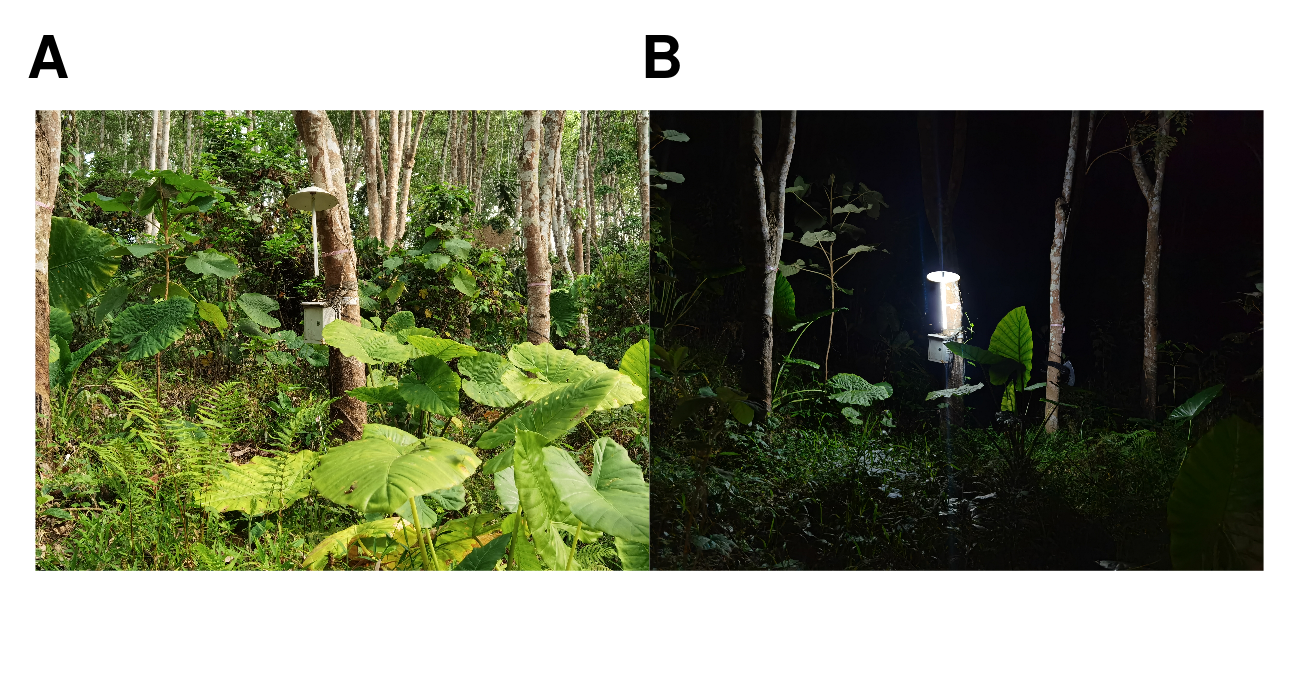
\includegraphics{../figs/merge.png}

\newpage

\begin{table}

\caption{Coefficients table}
\centering
\begin{tabular}[t]{r|l|r|>{}l}
\hline
X & Parameters & mean\_value & quantile\_interval\\
\hline
\multicolumn{4}{l}{\textbf{Melastoma\_candidum}}\\
\hline
\hspace{1em}1 & ALAN's effect & -0.0422 & [-0.1129, 0.0276]\\
\hline
\hspace{1em}2 & Daylight's effect & -0.0006 & [-0.0761, 0.0744]\\
\hline
\hspace{1em}3 & interaction & -0.0308 & [-0.0836, 0.0216]\\
\hline
\multicolumn{4}{l}{\textbf{Colocasia\_gigantea}}\\
\hline
\hspace{1em}4 & ALAN's effect & -0.1043 & \textbf{[-0.1458, -0.0621]}\\
\hline
\hspace{1em}5 & Daylight's effect & 0.0495 & \textbf{[0.0051, 0.0938]}\\
\hline
\hspace{1em}6 & interaction & -0.0120 & [-0.0428, 0.0195]\\
\hline
\end{tabular}
\end{table}

\textbf{Table. 1.} Results of Bayesian general linear mixed-effect
models testing the effects of artificial light at night, daylight and
interaction on experimental species. Significant effects (p \textless{}
0.05) are in bold.

\newpage



\end{document}
